\section{Wed, Feb 28th}
The computation of the expectation is
\begin{eqnarray*}
\Ex\{ \pi(r(1-\epsilon))\}&=&\begin{cases}
0&1-\frac{\lambda}{r}\leq 0\\
a^0-a^1r(1-\Ex\{\epsilon\})&\frac{1}{S\cdot UB}\left(1-\frac{\lambda}{r}\right)\geq 1\\
\frac{1}{(S\cdot UB)^2}\left(1-\frac{\lambda}{r}\right)^2(a^0-a^1r\left(1-\frac{1}{2}\left(1-\frac{\lambda}{r}\right)\right)\,&{\rm o.w.}
\end{cases}
\end{eqnarray*}
Note that this function is continuous.  The optimal value for $x\geq 0$ is given by
\begin{equation}
r^*(x)\in\argmax_r \lset \Ex\{ \pi(r(1-\epsilon))\}\mset r\geq x, \Ex\{ \pi(r(1-\epsilon))\}\geq 0\rset = \begin{cases}
\emptyset & x\geq \frac{a^0}{a^1}\frac{1}{1-\Ex\{\epsilon\}}\\
\frac{\lambda}{1-S\cdot UB}& 0\leq x<\frac{\lambda}{1-S\cdot UB}\\
x& \mbox{o.w}\end{cases}
\end{equation}
The function $\Ex\{ \pi(r(1-\epsilon))\}$ is depicted in Figure~(\ref{figExUt}).  From here it is easy to see that the optimum of the optimization problem depends on the values of $x$.

\begin{figure}[htbp] %  figure placement: here, top, bottom, or page
   \centering
   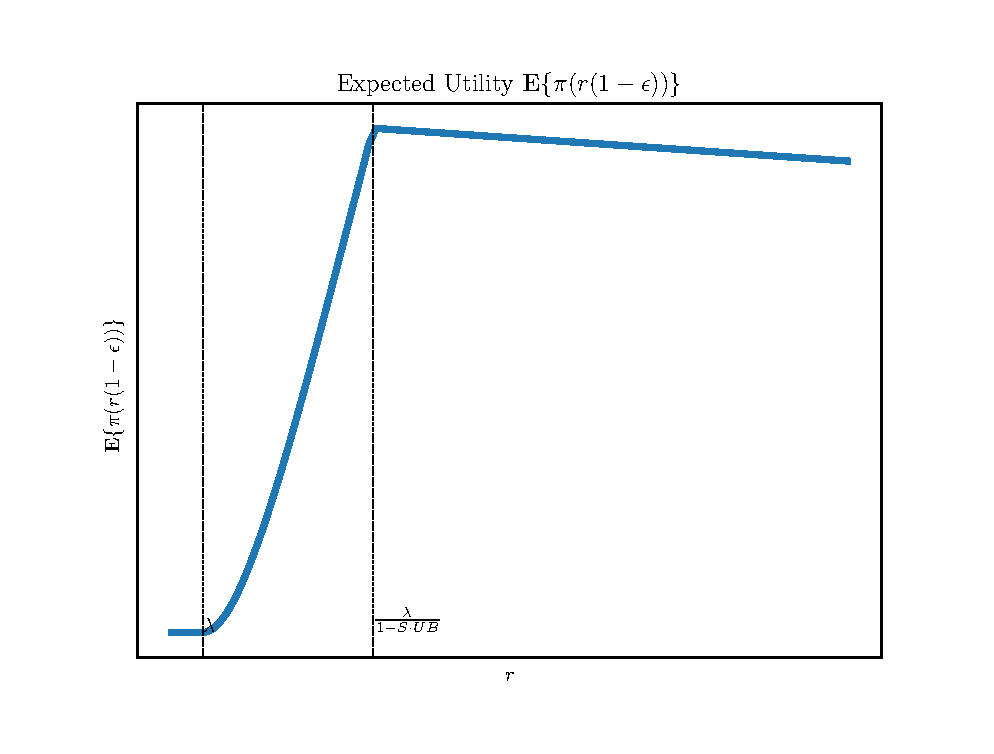
\includegraphics[width=0.7\textwidth]{ExpectedUt} 
   \caption{Expected utility}
   \label{figExUt}
\end{figure}

Finally, the optimal expected utility is given by
\begin{equation}\label{eqEPOpt}
\Ex\pi\{r^*(x)(1-\epsilon)\}=\begin{cases}
a^0-a^1x(1-\Ex\{\epsilon\})&\frac{\lambda}{1-S\cdot UB}\leq x\leq \frac{a^0}{a^1}\frac{1}{1-\Ex\{\epsilon\}}\\
a^0-a^1\frac{\lambda}{1-S\cdot UB}(1-\Ex\{\epsilon\})&0\leq x\leq \frac{\lambda}{1-S\cdot UB}\\
0&{\rm ow}
\end{cases}
\end{equation}
and it's depicted on Figure~(\ref{figOpExUt}).

\begin{figure}[htbp] %  figure placement: here, top, bottom, or page
   \centering
   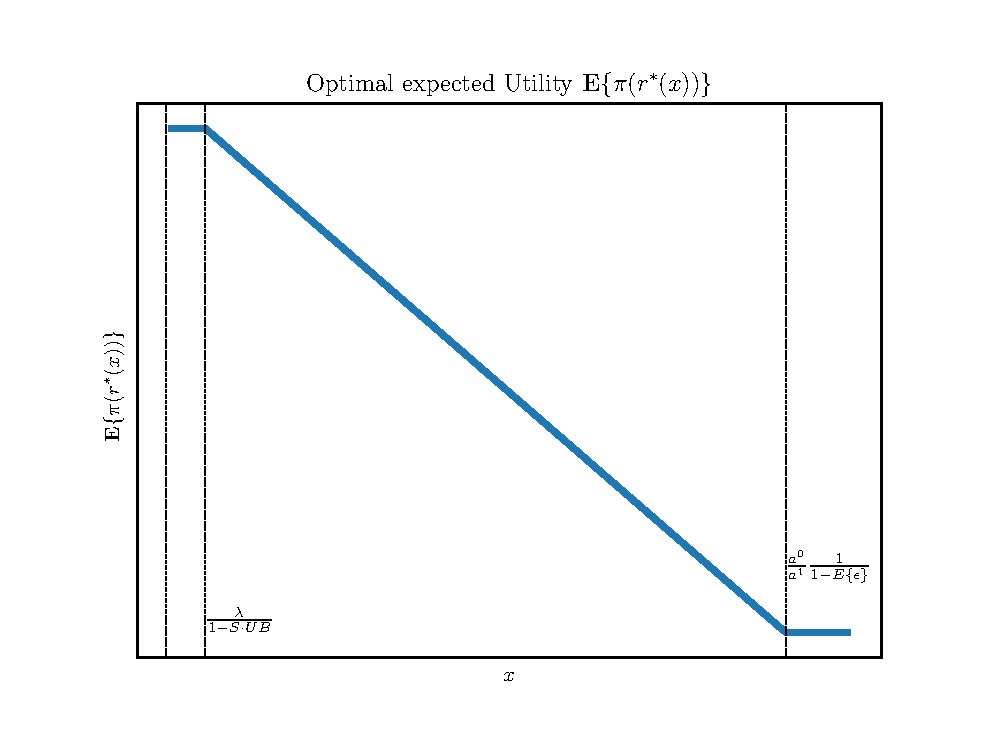
\includegraphics[width=0.7\textwidth]{OptExpUt} 
   \caption{Optimal Expected utility}
   \label{figOpExUt}
\end{figure}
